\chapter{Introduction}

Hardware components have been known to be extremely complex due to
concurrency. A system having concurrency indicates that independent
works can be done simultaneously, and it usually occurs as a name of
optimization. For example, instruction pipelining is one of
representative optimizations, which employes an instruction-level
parallelism to handle multiple executions at the same time. Concurrent
executions usually involve nondeterminism, since there is no fixed
sequence of execution for them. Nondeterminism is generally hard to
deal with, since all possible execution cases should be considered.

Modularity has been considered as an effective way to design and
understand such complex hardware components. Modularity indicates that
a complex hardware component can be constructed by composing simple
modules. Several Hardware Description Languages (HDLs) such as Verilog
or VHDL~\cite{verilog, vhdl} employ the notion of modules, each of
which acts as a small unit component.

Among various HDLs, \Bluespec{}~\cite{bsdef, bsref} allows designers
to develop hardware based not only on modularity, but also on the
prevalent paradigm called Guarded Atomic Actions
(GAAs)~\cite{daniel-gaa}. Even though a HDL allows to design hardware
in a modular manner, modules cannot be independently designed if they
are entangled with clock-timing issues. For instance, when two modules
are connected with wires and one module is optimized to need shorter
clock cycles, then the other module should follow that cycle, or the
optimized module should maintain the original clock even if it is
optimized.

Following the concepts of modularity and GAA, we have been defining a
framework called \Kami{}~\cite{kami-web}, which is for specifying,
verifying, and synthesizing \Bluespec{}-style hardware
components. \Kami{} presents a domain specific language similar to
Bluespec, and aims to prove properties of hardware automatically. In
order for such proofs, we also have defined formal semantics of the
\Kami{} language, based on modularity. The framework has been built on
the Coq proof assistant, hence verification can be performed by
mechanized proofs.

Modularity fits for scalable verification, especially with mechanized
proofs. In terms of verification, modularity indicates that complex
hardware components can be verified if each simple element is
verified. In many cases, we reuse such simple components for different
uses. From the perspective of proof, reusing a hardware component
implies that we can also reuse its related proofs. Thanks to the
modular semantics in \Kami{}, it is indeed possible to use the proof
of a component whenever it is used for the part of a design.

An important aspect of the modular semantics is that modules
communicate by labels. It is originated from the concept called
Labeled Transition System (LTS). Each module changes its internal
state and the corresponding label is generated during the state
transition. On the modular semantics, labels are method calls. In
other words, modules communicate by calling methods of other modules.
The modular semantics also take advantage of the LTS concept to define
behaviors of \emph{open systems}. Open systems have external
interactions, which cannot be figured out unless it is connected with
other modules which can respond to them.

\begin{figure}[t]
  \centering
  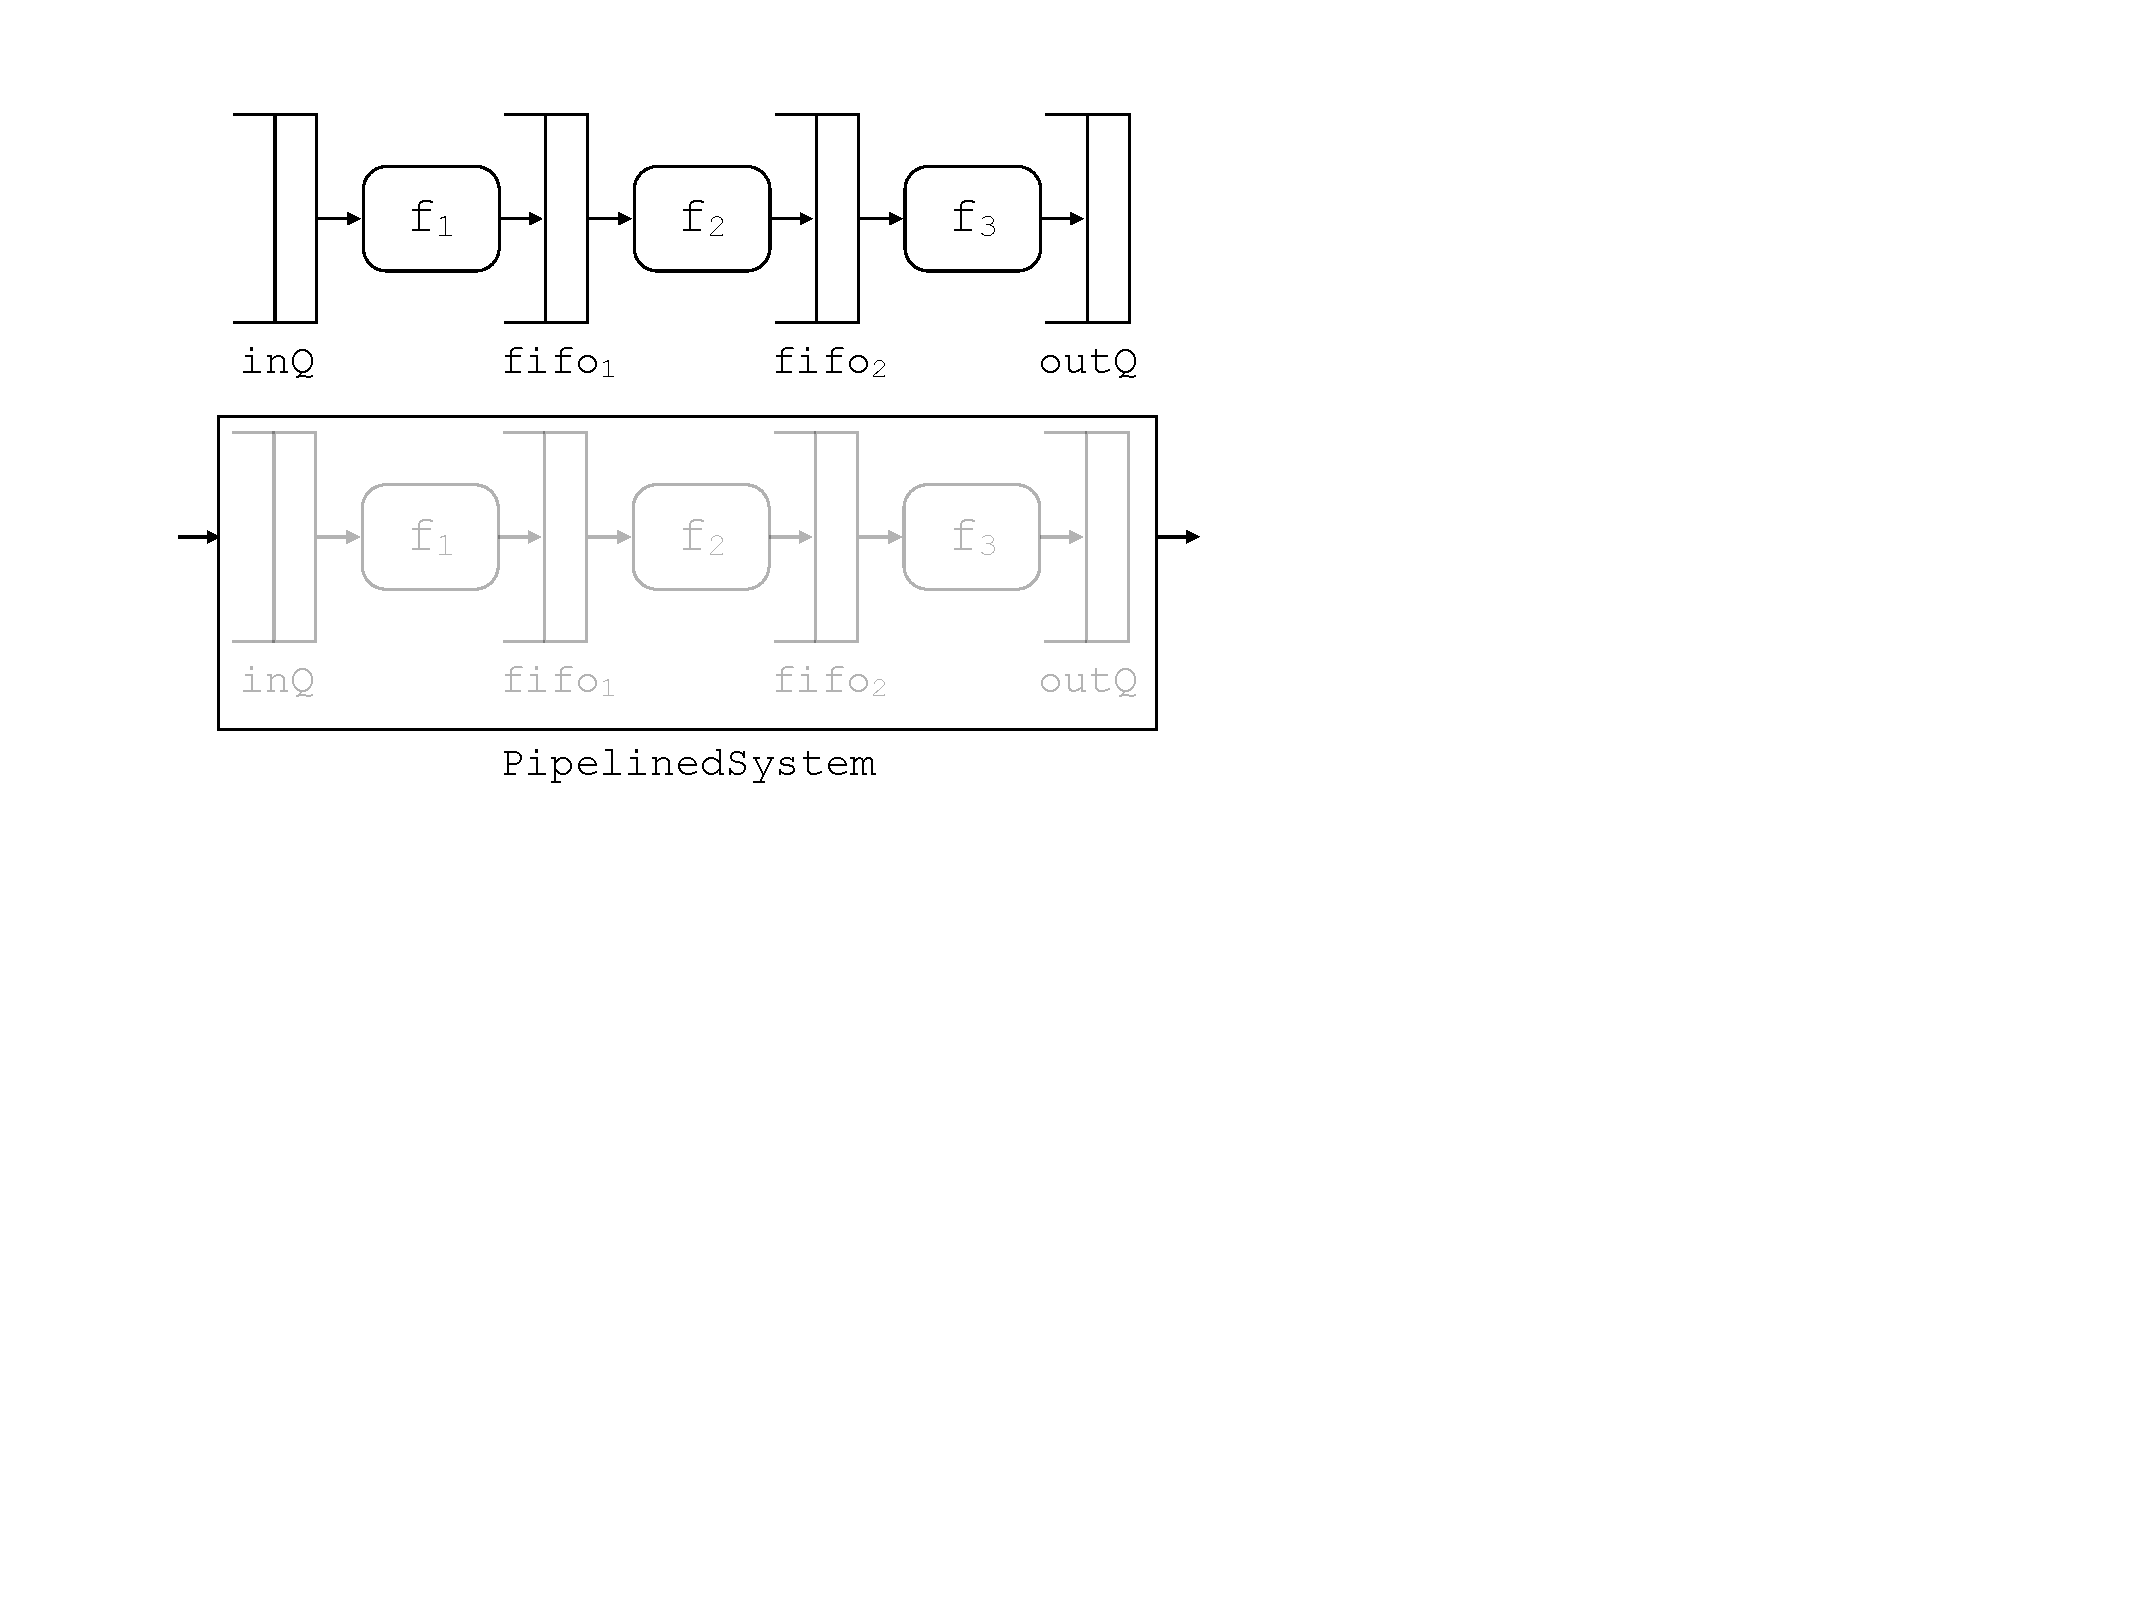
\includegraphics[width=0.6\textwidth]{figures/pipeline-internal.pdf}
  \caption{Internal states hidden by the module}
  \label{ex-modular-semantics-disadvantage}
\end{figure}

However, the modular semantics has an inherent weakness that it is
hard to track internal state changes by internal communications.
Consider a pipelined system, as shown in the upper part of
\reffig{ex-modular-semantics-disadvantage}. $\texttt{f}_1$,
$\texttt{f}_2$, and $\texttt{f}_3$ are modules which get an input from
the corresponding fifos $\texttt{inQ}$, $\texttt{fifo}_1$, and
$\texttt{fifo}_2$, respectively. When the system is built, modular
semantics abstract the system as a big module, in which only two
interfaces are revealed: one for input to $\texttt{inQ}$, and the
other for output from $\texttt{outQ}$ (as shown in the lower part of
the figure where internal modules are drawn vaguely). In this case,
when having information for an input and the output by the entire
system, how can we describe the \emph{internal state changes} in the
system? For instance, is $\texttt{fifo}_1$ storing an element for
given input and output? In modular semantics, we even cannot draw the
fact that the system is implemented by pipelines, since the semantics
are not defined by following execution paths, but by a series of local
communication among small modules.

A number of semantics, which do not have such a weakness, have been
defined but none of them was defined for open systems. In other words,
there have been no semantics which is able to define communication
with external modules. A big-step semantics along with the action
structures in \Bluespec{} have been defined~\cite{nirav-memocode}, but
it does not have a notion for external communications.

Hence, in this thesis, I present a new semantic approach, which is
based on inlining. Inlining semantics is defined for open hardware
systems and resolve the weakness by construction. The semantics uses a
static inlining operation to substitute internal calls to their method
bodies. This operator erases all internal calls in a module, so that
we do not need to care about internal communications.

An implication from the modular semantics to the inlining semantics is
also formally proven, thus it can be used in order to efficiently
prove properties of hardware. Since the two semantics does not have
equal capabilities, we give the implication proof saying that the
modular semantics imply the inlining semantics.

To sum up, the main contributions of this thesis are:
\begin{itemize}
\item To define a new semantic approach based on inlining, for open
  hardware systems.
\item To prove the implication from the modular semantics to the
  inlining semantics.
\end{itemize}

\paragraph{Overview}

The thesis is organized as follows: \refchap{chap:backgrounds}
introduces a number of prerequisites to understand the hardware design
concept of \Bluespec{}. Related works are also provided to compare
previous approaches to define hardware semantics.
\refchap{chap:semantics} presents the two semantics used in the
\Kami{} framework: modular and inlining
semantics. \refchap{chap:implication} compares capability of each
semantics and presents the implication proof between them. Lastly, we
draw conclusions and give future works in \refchap{chap:conclusions}.

